\documentclass[10pt,conference,compsocconf]{IEEEtran}

%\usepackage{times}
%\usepackage{balance}
\usepackage{url}
\usepackage{graphicx}
\usepackage{hyperref}
\usepackage{color}

\newcommand{\todo}[1]{}
\renewcommand{\todo}[1]{{\color{red} TODO: {#1}}}

\newcommand{\pisch}[1]{\textit{\textcolor{blue}{pisch: #1}}}

\begin{document}
\title{CIL 2018: Text Sentiment Classification}

\author{
  Aryaman Fasciati, Nikolas G\"obel, Philip Junker, Pirmin Schmid\\
  The Optimists\\
  Department of Computer Science, ETH Zurich, Switzerland
}

\maketitle

\begin{abstract}
  In this work we consider the task of classifying tweets by
  sentiment. In particular we want to determine whether a given tweet,
  which has been stripped of emoticons, used to include a positive
  smiley ``:)'' or a negative smiley ``:(''. We present a stacked RNN
  model trained on GloVe word embeddings. Our model achieves a
  classification accuracy of 86.6\%.
\end{abstract}


\section{Introduction}
The global prevalence of social media has enabled a massive amount of users
to publicly voice their opinions and interact with each other.
Microblogging services like Twitter\footnote{www.twitter.com} make it
very easy for users to comment on current events, tell other users about their
lives, and discuss the products and services they use.
This data can be analysed for sentiments and opinions and can be used for
various purposes, such as brand monitoring or stock market prediction.

The goal of this project is to build a sentiment classifier that
predicts whether a Twitter tweet used to include a positive smiley :) or
a negative smiley :(, based on the remaining text.

Our first baseline uses random forests and achieved an accuracy of
72\%. Our second baseline uses a Recurrent Neural Network (RNN) model
with an accuracy of \todo{rnn-baseline-accuracy}.

In a third model, we refined our second baseline, incorporating
\todo{describe novel approach}, in a RNN-based approach. This model
achieved \todo{\%} accuracy.


\section{Related Work}

Recurrent neural networks with their applicability to
sequence-to-sequence tasks have been used across many tasks,
especially in the NLP domain, such as generating text (\todo{Sutskever
  et al.}). Although RNNs seem to be primarily used for problems more
complex than binary classification, we were interested in exploring
the application of short-term memory to our task. This can be achieved
via the Long short-term memory (LSTM) or Gated recurrent unit (GRU)
variants of RNNs. Both have found extensive use in practical
applications, such as \todo{cite
  https://ai.googleblog.com/2016/05/chat-smarter-with-allo.html}.

\section{Models}

\subsection{First Baseline (B1)}

Our first baseline uses a random forest model with unlimited
max\_depth and 20 estimators. We used the random forest implementation
provided with the scikit-learn library \cite{scikit-learn}.  The
classifier is trained on tweet embeddings, derived by computing the
mean over all embedding vectors of the words contained within it. This
approach does not differentiate between permutations of similar
words. It also assigns equal weight to every word. Words that are not
in the vocabulary are ignored. Word embeddings are provided by the
GloVe \cite{glove} project from Stanford, pre-trained on two billion
tweets. In addition to that, tweets were pre-processed with a slightly
adapted version of the preprocessor script provided by Stanford.

This model achieved an accuracy of 72\%.

\subsection{Second Baseline (B2)}

For the second baseline, we trained a stacked, recurrent neural
network. Two GRU cells were stacked; a hidden state size of 384 was used.
In contrast to the random forest baseline, tweet embeddings
were not aggregated in any way from their words. Rather, the network
was trained on matrices of dimension \(word\_count_{tweet} \times 200\).
Words not known in the embedding vocabulary were ignored.
Statistical analysis of the provided data in \autoref{fig:wordcount} shows that
the majority ($>$98\%) of tweets have less than 30 words.
Tweets longer than that were ignored during training and shortened for prediction,
whereas shorter tweets were padded.

All output of the RNN was used as input of a single layer fully connected NN
to 2 nodes with a sigmoid activation function.
Argmax was used to determine the sentiment.
Loss was calculated with sparse softmax cross entropy with logits and
an Adam optimizer was used for learning with clipped gradient at 10
and a learning rate of $10^{-4}$.
In total, the model was trained for 4 epochs on Leonhard.
98\% of the training data was used for training; 2\% was used for evaluation.

Smaller and larger hidden state sizes were tested but resulted in
lower accuracy. Additonally, we experimented with LSTM cells, which did not give us
a higher score than with GRU cells.
All outputs of the RNN were used as input of the NN to bring more state
information into the final classifier step. Using only the final hidde
state has been tested and gave lower accuracy.
And finally, a small NN was used to handle the binary classification from the RNN 
state to allow also for non-linear transformation in contrast to the classic 
transformation with a matrix multiplication and potentially adding of a
bias offset.

\pisch{not yet sure about this discussion points here}
In contrast to B1, this model does take word order into account
and allows for different weights to be assigned to certain,
sentiment-implying words, during training. Intuitively, we would
expect the latter to result in significantly higher classification
accuracy, compared to the random forest model. It is not as clear,
whether taking word order into account during training is important
for the task of sentiment classification and would thus dilute inputs
in a sense.

This model achieved an accuracy of 85\%.

\begin{figure}[h!]
  \centering
  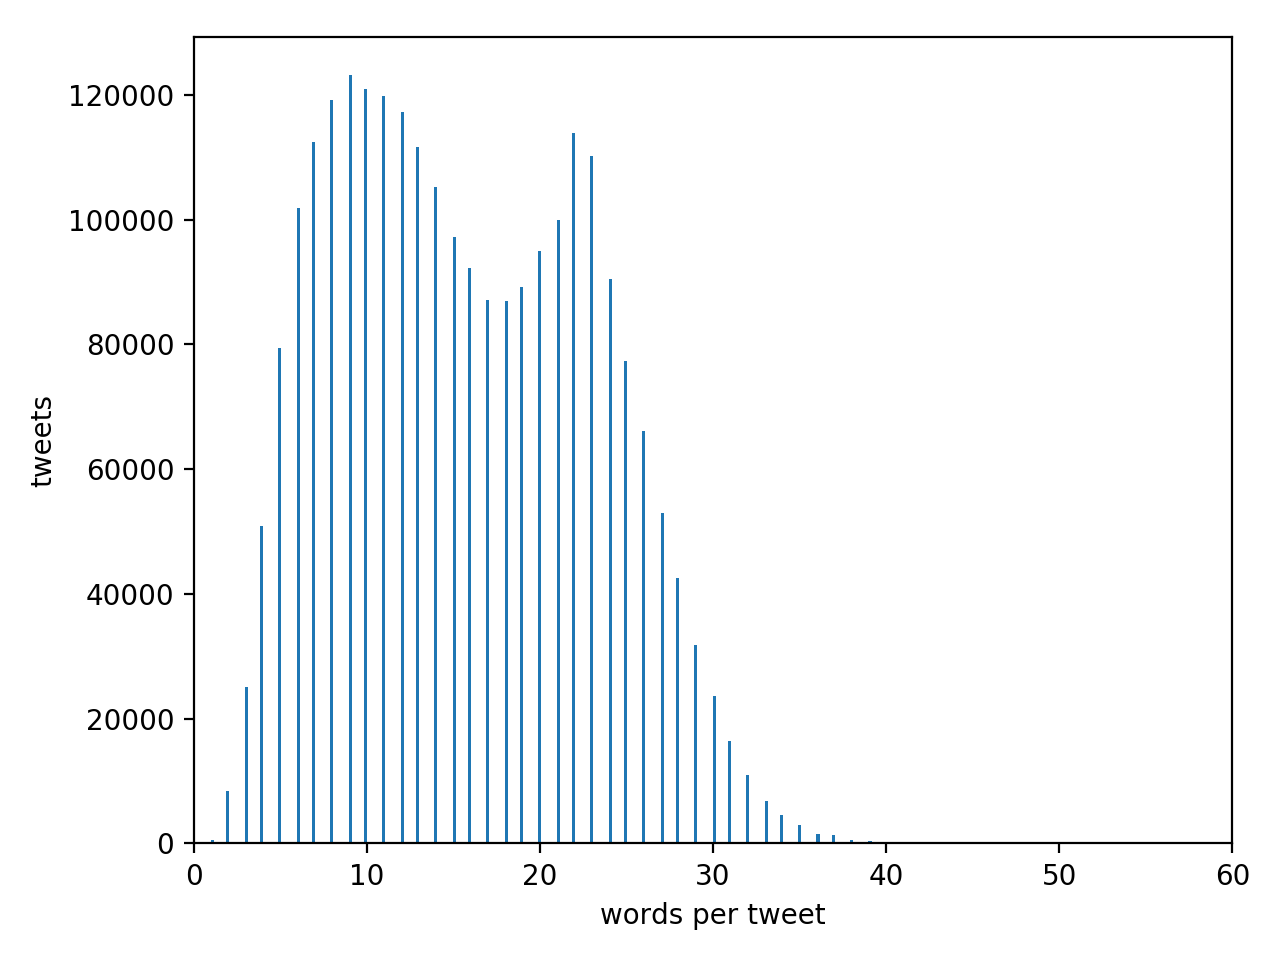
\includegraphics[scale=0.53]{word_count_histogram.png}
  \caption{Word Count Distribution}
  \label{fig:wordcount}
\end{figure}


\subsection{Our Model}

For our final model, we decided to expand on the promising RNN
approach taken in baseline B2. We can consider the RNN output to
represent learned tweet features, which bear significance for
sentiment classification. Consequently, we wanted to re-combine these
features in a structure-preserving, context-sensitive
manner. Convolutional neural networks fit this bill and in addition
possess the property of being invariant w.r.t
translation. Intuitively, this sounded useful to the task at hand,
because we expect certain word sequences to indicate sentiment
independent of where they appear inside a tweet.

We therefore introduced two one-dimensional convolution layers each
followed by a one-dimensional max-pooling layer. We chose convolution
window sizes of six and four respectively, with no bias and ReLu
activation. The max-pooling layers aggregate each pooling window into
a single scalar. We chose a window size of two and strides of two for
both layers. Outputs for every window are concatenated and passed on
to a fully connected rectifier. In order to lessen the impact of
overfitting, we apply a dropout rate of 0.4 during training.

The final outputs are then fed into a two-unit layer, each unit
indicating one of the two possible sentiments. Overall classification
output is then obtained by applying the \texttt{argmax} function.

\section*{Acknowledgements}

The authors wish to express their gratitude to the Euler and Leonhard
clusters at ETH, whose unwavering computational effort this project
could not have done without.

\bibliographystyle{IEEEtran}
\bibliography{TheOptimists-literature}
\end{document}
